\documentclass[aspectratio=169,11pt]{beamer}

% ============================================================
% Theme
% ============================================================
\usetheme{Madrid}
\usecolortheme{seahorse}
\setbeamertemplate{navigation symbols}{}

% Optional safe progress indicator (never breaks):
\setbeamertemplate{footline}[frame number]

% ============================================================
% Encoding
% ============================================================
\usepackage[utf8]{inputenc}
\usepackage[T1]{fontenc}
\usepackage{lmodern}

% ============================================================
% Packages
% ============================================================
\usepackage{amsmath}
\usepackage{xcolor}
\usepackage{listings}
\usepackage{tikz}
\usetikzlibrary{positioning,arrows.meta,patterns}

% ============================================================
% Listings (Java)
% ============================================================
\lstset{
	language=Java,
	basicstyle=\ttfamily\small,
	frame=single,
	breaklines=true,
	columns=fullflexible,
	keywordstyle=\color{blue},
	commentstyle=\color{gray!70!black},
	stringstyle=\color{red!70!black},
	showstringspaces=false,
	backgroundcolor=\color{gray!5}
}

% Small helper: safe “code box” usable inside columns (matches listings)
\newcommand{\codebox}[1]{%
	\begingroup
	\setlength{\fboxsep}{6pt}%
	\colorbox{gray!5}{\ttfamily\small #1}%
	\endgroup
}

% ============================================================
% Title
% ============================================================
\title{Concurrency \& Distributed Systems}
\subtitle{Week 2 --- Part 3: sleep() vs join()}
\author{Dr. Mohamad Aoude}
\institute{Lebanese University \\ Faculty of Engineering}
\date{\today}

% ============================================================
\begin{document}
	
	% ============================================================
	\begin{frame}
		\titlepage
	\end{frame}
	
	% ============================================================
	\begin{frame}
		\frametitle{A Fundamental Coordination Question}
		
		\begin{block}{Scenario}
			Thread A must finish before Thread B continues.
		\end{block}
		
		\vspace{5mm}
		
		Should we:
		\begin{itemize}
			\item Delay using \texttt{sleep()}?
			\item Coordinate using \texttt{join()}?
		\end{itemize}
		
		\vspace{6mm}
		
		\begin{center}
			\Large
			Clocks measure time. \\[2mm]
			Synchronization observes state.
		\end{center}
		
	\end{frame}
	
	% ============================================================
	\begin{frame}
		\frametitle{Core Distinction}
		
		\begin{columns}
			
			\column{0.48\textwidth}
			\textbf{sleep()}
			
			\begin{itemize}
				\item Pauses current thread
				\item Time-based
				\item Independent of other threads
				\item TIMED\_WAITING state
			\end{itemize}
			
			\column{0.48\textwidth}
			\textbf{join()}
			
			\begin{itemize}
				\item Waits for target thread
				\item Completion-based
				\item Observes thread state
				\item WAITING state
			\end{itemize}
			
		\end{columns}
		
		\vspace{5mm}
		
		\begin{center}
			\Large
			Time vs State
		\end{center}
		
	\end{frame}
	
	% ============================================================
	\begin{frame}[fragile]
		\frametitle{Broken Coordination: Concrete Failure}
		
		\begin{lstlisting}
			// Shared state
			static int counter = 0;
			
			Thread worker = new Thread(() -> {
				for (int i = 0; i < 1_000_000; i++) {
					counter++;
				}
			});
			
			worker.start();
			
			// WRONG: guess a delay
			Thread.sleep(10);  // throws InterruptedException
			
			System.out.println(counter);
		\end{lstlisting}
		
	\end{frame}
	
	% ============================================================
	\begin{frame}
		\frametitle{Why This Fails}
		
		\begin{itemize}
			\item May work on fast machine
			\item Fails under CPU contention
			\item Fails during GC pauses
			\item Fails with OS scheduling variation
			\item Fails in virtualized/cloud environments
		\end{itemize}
		
		\vspace{6mm}
		
		\begin{block}{Reality}
			Timing-based coordination is probabilistic, not deterministic.
		\end{block}
		
	\end{frame}
	
	% ============================================================
	\begin{frame}
		\frametitle{Before/After Output (What Students Actually See)}
		
		\begin{block}{Without join() (timing guess)}
			\ttfamily\small
			457821 \quad \textit{(wrong: worker still running)}
		\end{block}
		
		\vspace{4mm}
		
		\begin{block}{With join() (completion-based)}
			\ttfamily\small
			1000000 \quad \textit{(correct: worker finished)}
		\end{block}
		
		\vspace{3mm}
		
		\begin{center}
			\Large
			This is not ``ordering cosmetics'' — it is incorrect results.
		\end{center}
		
	\end{frame}
	
	% ============================================================
	\begin{frame}
		\frametitle{Why sleep() Cannot Synchronize}
		
		\begin{itemize}
			\item Does NOT observe other threads
			\item Does NOT wait for completion
			\item Does NOT guarantee ordering
			\item Does NOT establish happens-before
			\item Sensitive to load and scheduling
		\end{itemize}
		
	\end{frame}
	
	% ============================================================
	\begin{frame}[fragile]
		\frametitle{Correct Coordination with join()}
		
		\begin{lstlisting}
			worker.start();
			
			worker.join(); // throws InterruptedException
			
			System.out.println(counter);
		\end{lstlisting}
		
		\vspace{4mm}
		
		\begin{block}{Interrupt Handling (Production Rule)}
			If interrupted, restore the interrupt status:
			\texttt{Thread.currentThread().interrupt();}
		\end{block}
		
	\end{frame}
	
	% ============================================================
	\begin{frame}
		\frametitle{What join() Actually Does}
		
		\begin{itemize}
			\item Calling thread blocks
			\item JVM checks if target thread is alive
			\item If alive → WAITING
			\item If already finished → returns immediately
		\end{itemize}
		
		\vspace{4mm}
		
		\begin{block}{Implementation Insight (Most JVMs)}
			In many JVM implementations, \texttt{join()} is built using
			\texttt{wait()/notifyAll()} on the \texttt{Thread} object's monitor.
		\end{block}
		
	\end{frame}
	
	% ============================================================
	\begin{frame}
		\frametitle{Execution Timeline (State Becomes Visible)}
		
		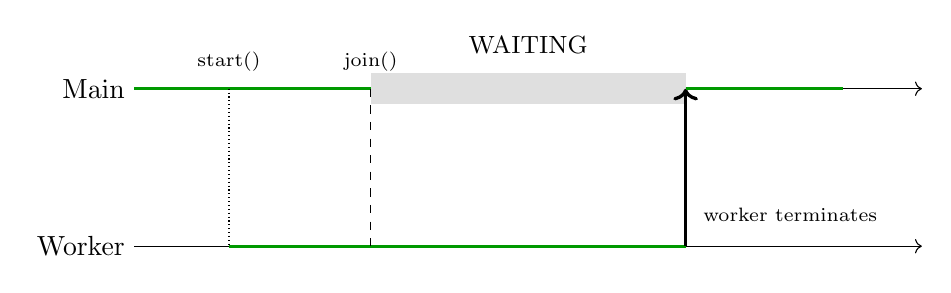
\begin{tikzpicture}
			
			% Axes
			\draw[->] (0,0) -- (10,0);
			\draw[->] (0,-2) -- (10,-2);
			
			\node[left] at (0,0) {Main};
			\node[left] at (0,-2) {Worker};
			
			% Main active segment (green)
			\draw[very thick, green!60!black] (0,0) -- (3,0);
			
			% Start marker for worker
			\draw[densely dotted] (1.2,0) -- (1.2,-2);
			\node[anchor=south] at (1.2,0.1) {\scriptsize start()};
			\pause
			
			% Worker active (green)
			\draw[very thick, green!60!black] (1.2,-2) -- (7,-2);
			
			% Join marker
			\draw[dashed] (3,0) -- (3,-2);
			\node[anchor=south] at (3,0.1) {\scriptsize join()};
			\pause
			
			% Main waiting region (gray fill)
			\fill[gray!25] (3,-0.2) rectangle (7,0.2);
			\node at (5,0.55) {\small WAITING};
			\pause
			
			% Resume arrow at termination
			\draw[->, very thick] (7,-2) -- (7,0);
			\node[anchor=west] at (7.1,-1.6) {\scriptsize worker terminates};
			
			% Main resumes (green)
			\draw[very thick, green!60!black] (7,0) -- (9,0);
			
		\end{tikzpicture}
		
	\end{frame}
	
	% ============================================================
	\begin{frame}
		\frametitle{Memory Visibility Guarantee}
		
		\begin{itemize}
			\item \texttt{join()} creates a happens-before relationship
			\item Thread termination happens-before successful return from \texttt{join()}
		\end{itemize}
		
		\vspace{5mm}
		
		\begin{block}{Precise Rule}
			All writes by worker before termination become visible after \texttt{join()} returns.
		\end{block}
		
		\vspace{2mm}
		\scriptsize (Formal rules: JLS \S 17.4.5)
	\end{frame}
	
	% ============================================================
	\begin{frame}[fragile]
		\frametitle{join(long millis)}
		
		\begin{lstlisting}
			worker.join(1000);
		\end{lstlisting}
		
		\begin{itemize}
			\item Waits up to 1 second
			\item Returns earlier if worker finishes
			\item If timeout expires, worker may still be alive
			\item No completion guarantee
		\end{itemize}
		
	\end{frame}
	
	% ============================================================
	\begin{frame}
		\frametitle{Lifecycle Mapping}
		
		\begin{itemize}
			\item \texttt{sleep()} → TIMED\_WAITING
			\item \texttt{join()} → WAITING
			\item Worker terminates → Main becomes RUNNABLE
		\end{itemize}
		
	\end{frame}
	
	% ============================================================
	\begin{frame}[fragile]
		\frametitle{Fork-Join Pattern}
		
		\begin{lstlisting}
			t1.start();
			t2.start();
			
			t1.join();
			t2.join();
		\end{lstlisting}
		
		\begin{itemize}
			\item Parallel execution
			\item Join point enforces completion
			\item Classic fork-join structure
		\end{itemize}
		
	\end{frame}
	
	% ============================================================
	\begin{frame}
		\frametitle{When Is sleep() Acceptable? (With Caveats)}
		
		\begin{itemize}
			\item Rate limiting / backoff (e.g., retry after failure)
			\item Simulation / demos (explicitly labeled)
			\item UI animation timing (not correctness-critical)
			\item Testing support (with clear disclaimers)
		\end{itemize}
		
		\vspace{4mm}
		
		\begin{block}{Rule}
			Never use \texttt{sleep()} for correctness-critical coordination.
		\end{block}
		
	\end{frame}
	
	% ============================================================
	\begin{frame}
		\frametitle{Deep Conceptual Contrast}
		
		\begin{columns}
			
			\column{0.48\textwidth}
			\textbf{Time-Based}\\[2mm]
			\codebox{sleep(5000);}\\[2mm]
			\small ``I wait 5 seconds.''
			
			\column{0.48\textwidth}
			\textbf{State-Based}\\[2mm]
			\codebox{worker.join();}\\[2mm]
			\small ``I wait for worker.''
			
		\end{columns}
		
		\vspace{6mm}
		
		\begin{center}
			\Large
			Synchronization is event-driven, not clock-driven.
		\end{center}
		
	\end{frame}
	
	% ============================================================
	\begin{frame}
		\frametitle{Reflection Questions}
		
		\begin{enumerate}
			\item If worker takes 10s on a fast machine and 11s on a slow one, does sleep(10000) always work? Why?
			\item Would sleep(60000) be safe in production?
			\item What exact memory guarantee does join() provide?
			\item How is join() related to wait()/notifyAll()?
			\item Why is event-based coordination fundamentally safer?
		\end{enumerate}
		
	\end{frame}
	
	% ============================================================
	\begin{frame}
		\frametitle{Summary}
		
		\begin{itemize}
			\item \texttt{sleep()} delays execution
			\item \texttt{join()} coordinates completion
			\item \texttt{join()} guarantees ordering
			\item \texttt{join()} guarantees memory visibility
			\item \texttt{sleep()} is NOT synchronization
		\end{itemize}
		
		\vspace{5mm}
		
		\begin{block}{One Rule to Remember}
			Never coordinate threads using time. Always coordinate using state.
		\end{block}
		
	\end{frame}
	
\end{document}
